\documentclass[11pt]{article}
\usepackage{color}
\usepackage{graphicx}
\usepackage{amsmath,amsthm,amssymb,multirow,paralist}
\usepackage[margin=0.8in]{geometry}
\usepackage{hyperref}

\begin{document}

\begin{center}
{\Large \textbf{COM S 5730 Homework 3}}\\

\linethickness{1mm}\line(1,0){498}

\begin{enumerate}
\item Please put required code files and report into a
compressed file ``HW3\_FirstName\_LastName.zip''
\item Unlimited number of submissions are
allowed on Canvas and the latest one will be graded.
\item Due: \textbf{Tuesday Oct. 15, 2024 at 11:59pm.}
\item {\color{red} No later submission is accepted.}
\item Please read and follow submission instructions. No exception
will be made to accommodate incorrectly submitted files/reports.
\item All students are required to typeset their reports using
latex. Overleaf
(\url{https://www.overleaf.com/learn/latex/Tutorials}) can be a
good start.
\end{enumerate}

\linethickness{1mm}\line(1,0){498}

\end{center}

%%%%%%%%%%%%%%%%%%%%%%%%%%%%%%%%%%%%%%%%%%%%%%%%%%%%%%%%%%%%%%%%%%%%%%%%%%%%%%%

%%%%%%%%%%%%%%%%%%%%%%%%%%%%%%%%%%%%%%%%%%%%%%%%%%%%%%%%%%%%%%%%%%%%%%%%%%%%%%%


\begin{enumerate}

\item (15 points) You are provided with a training set of
examples (see Figure~\ref{fig:tree}). Which feature will you pick
first to split the data as per the ID3 decision tree learning
algorithm? Show all your work: compute the information gain for
all the four attributes and pick the best one.

\begin{figure*}[ht]\label{fig:tree}
\begin{center}
    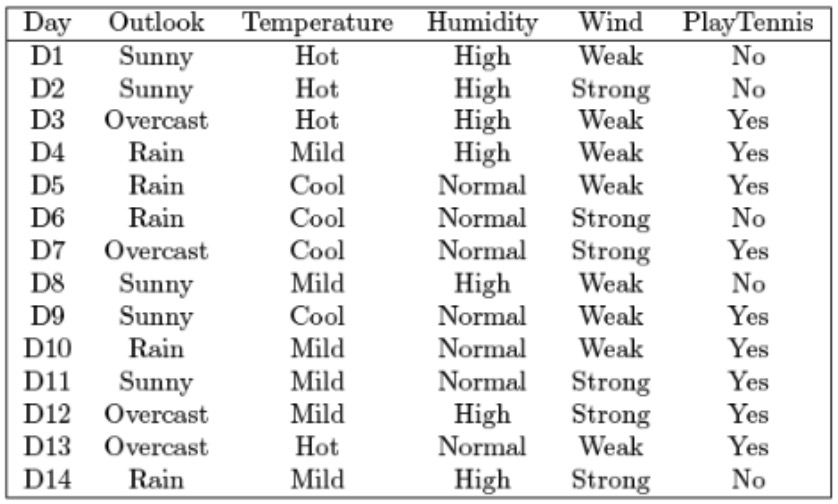
\includegraphics[width=0.6\textwidth]{tree.jpg}
    \caption{Table with training examples. Each row corresponds
    to a single training example. There are four features,
    namely, outlook, temperature, humidity, and wind.
    ``PlayTennis'' is the class label.}
\end{center}
\end{figure*}

\item (15 points) We know that we can convert any decision tree
into a set of if-then rules, where there is one rule per leaf
node. Suppose you are given a set of rules $R = \{r_1, r_2,
\dots, r_k\}$, where $r_i$ corresponds to the $i^{th}$ rule.
{\color{red} These rules are valid and complete, which means
there is no conflicting rules. You can always obtain a prediction
based on these rules.} Is it possible to convert the rule set $R$
into an equivalent decision tree? Explain your construction or
give a counterexample.


\item (20 points) Suppose $\boldsymbol x = [x_1, x_2, \dots,
x_d]$ and $\boldsymbol z = [z_1, z_2, \dots, z_d]$ be two points in
a high-dimensional space (i.e., $d$ is very large).

\begin{enumerate}
    \item (10 points) Try to prove the following, where the
    right-hand side quantity represent the standard Euclidean
    distance.
    \begin{align*}
        \left(\frac{1}{\sqrt{d}}\sum_{i=1}^d x_i - \frac{1}{\sqrt{d}} \sum_{i=1}^d z_i \right)^2 \le
        \sum_{i=1}^d \left(x_i - z_i\right)^2
    \end{align*}

    \textbf{Hint: } Use Jensen’s inequality – If $X$ is a random
    variable and $f$ is a convex function, then $f(E[X]) \le
    E[f(X)]$.

    
    \item (10 points) We know that the computation of nearest
    neighbors is very expensive in the high-dimensional space.
    Discuss how we can make use of the above property to make the
    nearest neighbors computation efficient?


\end{enumerate}

\item (50 points) \textbf{Car Evaluation}: You will
build a Car Evaluation classifier. This classifier will be
used to classify the condition of a car.

The data: car\_evaluation.csv. This is the data
consisting of car evaluations. 

\begin{enumerate}
\item (20 points) Implement the ID3 decision tree learning
algorithm that we discussed in the class. The key step in the
decision tree learning is choosing the next feature to split on.
Implement the information gain heuristic for selecting the next
feature. Please see lecture notes or
\url{https://en.wikipedia.org/wiki/ID3_algorithm} for more
details.

\item (20 points) Implement the decision tree pruning algorithm
discussed in the class (via validation data).

\item (10 points) Compute the accuracy of decision tree and
pruned decision tree on validation examples and testing examples.
List your observations by comparing the performance of decision
tree with and without pruning.

\end{enumerate}


\end{enumerate}

\end{document}
